% <- percent signs are used to comment
\documentclass[12pt]{article}

%%%%%% PACKAGES - this part loads additional material for LaTeX %%%%%%%%%
% Nearly anything you want can be done in LaTeX if you load the right package 
% (search ctan.org or google it if you are looking for something).  We will load
% here a few that we need for this document or that we expect you to need later.

% The next 3 lines are needed to fix shortcomings of TeX that only make sense given its 40-year history ...
% Simple keep and ignore.
\usepackage[utf8]{inputenc}
\usepackage[T1]{fontenc}
\usepackage{lmodern}


% Custom margins (and paper sizes etc.) because LaTeX else wastes much space
\usepackage[margin=1in]{geometry}

% The following packages are created by the American Mathematical Society (AMS)
% and provide lots of tools for special fonts, symbols, theorems, and proof
\usepackage{amsmath,amsfonts,amssymb,amsthm}
% mathtools contains many detail improvements over ams and core tex
\usepackage{mathtools}

% graphicx is required for images
\usepackage{graphicx}

% enumitem used for customizing enumerations
\usepackage[shortlabels]{enumitem}

% tikz is the package used for drawing, in particular for drawing trees. You may also find simplified packages like tikz-qtree and forest useful
\usepackage{tikz}

% hyperref allows links, urls, and many other PDF tricks.  We load it here
%          in such a way that the PDF file has info about it
\usepackage[%
pdftitle={CS240 Assignment 0},%
hidelinks,%
]{hyperref}


%%%%%% COMMANDS - here you can define your own LaTeX-commands %%%%%%%%%

%%%%%% End of Preamble %%%%%%%%%%%%%

\begin{document}
	
	\begin{center}
		{\Large\textbf{University of Waterloo}}\\
		\vspace{3mm}
		{\Large\textbf{CS240, Fall 2021}}\\
		\vspace{2mm}
		{\Large\textbf{Assignment 0}}\\
		\vspace{3mm}
		\textbf{Due Date: Wednesday, Sept 15, 2021 at 5:00pm}
	\end{center}
	
	Please read
	\url{http://www.student.cs.uwaterloo.ca/~cs240/f21/guidelines/guidelines.pdf}
	for guidelines on submission.  For problems 1\,--\,6, submit your
	solutions electronically using MarkUs.
	This assignment is worth up to 6 bonus marks, which will be added to
	your total mark (raw score) for assignment 1.
	
	
	%\section marks off a section, 
	% adding an * at the end does not number the section and suppresses it in the table of contents
	\section*{Introduction}
	
	A0 is designed to introduce you to \LaTeX.
	We strongly encourage students to create all their assignment solutions using \LaTeX,
	as it will strongly benefit both you and your markers. While \LaTeX{} is not required for CS240,
	non-\LaTeX{} submissions are expected to be of comparable presentation and sufficiently
	messy, hard-to-read solutions%
	\footnote{%
		What exactly ``hard-to-read'' means is at the marker's interpretation~-- 
		if you want to be sure it is readable, use \LaTeX!%
	} 
	may be penalized. 
	
	% An empty line starts a new paragraph.
	
	Learning \LaTeX{} is a great asset 
	to have for any course, and also especially for those of you planning to go into academia.
	As a beginner in \LaTeX, like in HTML, it is best to start with an example. 
	(And like HTML, \LaTeX{} comes with considerable legacy; some features are clearly deprecated,
	but still exist for backward compatibility)
	
	To complete the problems below, open the 
	\LaTeX{} file used to make this PDF. Inside the file you will find the code used to write this
	file along with comments explaining the code to help you get through the assignment. If you get
	stuck there are also many on-line resources you can use;
	in particular \url{http://tex.stackexchange.com} is a valuable resource.
	Searching for ``fraction example \LaTeX'' 
	is acceptable; searching for ``\LaTeX{} proof of summation from 1 to n'' 
	is \textbf{not} acceptable (academic violation). 
	
	To compile the .tex file provided simply type ``\texttt{pdflatex a0.tex}'' 
	in the school's Linux environment. \LaTeX{} compilers are also free to download on-line.
	\textbf{Submit both a0.pdf and a0.tex to MarkUs}.
	
	
	% Clearpage starts a new page, unless (by chance) a page break happens to be here anyway
	\clearpage
	
	\section{Assignment Guidelines}
	% We can assign a label to each section (and also many other things, such as 
	% figures, lemmas, ...) and then refer to them.  For this to be correct, the
	% file must be translated twice.
	\label{sec:assignment-guidelines}
	
	At the top of this page is the URL to the assignment guidelines for CS240, it can also be found from the course webpage from the Assignments tab. Please answer the following questions about the assignment guidelines:
	
	% "itemize" creates a bulleted list, "enumerate" creates a list with numbers.
	% However, enumerate by default uses 1,2,..., but we want a,b,..., so override
	% the options
	\begin{enumerate}[a)] 
		\item If an assignment question asks you to design an algorithm, what are the three other things you must do in addition to describing/writing the pseudocode for the algorithm?
		
		\begin{itemize}
			\item Describe the main idea first in words
			\item Give a correctness proof or justification, and
			\item Include an analysis (usually, of the running time).
		\end{itemize}	
		
		\item For programming questions, what can you use to read input? \\ What can you use to output the answer?
		
		\begin{itemize}
			\item For programming questions, programs should read from the standard input stream(std::cin), and write to the standard output stream(std::cout).
		\end{itemize}
		
	\end{enumerate}
	
	\section{Mathematics}
	In CS240, you will be using many mathematical concepts. It is important to be able to typeset mathematics in your assignments. This will include sums, fractions, subscripts \& superscripts, etc. \\
	Example: 
	
	% \[ ... \] means a math-equation that is bigger and centered
	\[ \bar{f}(n) \coloneqq \sqrt {\sum_{i=0}^{\lg n} 4^i \left ( \frac{n_0}{2^i} \right )^{\theta}}. \]
	In order to practice this skill, write a proof showing: \[ \sum_{i=1}^n i = \frac {n(n+1)} {2} \]
	
	{\itshape
		Hint: For short formulas, we use inline math surrounded by \texttt{\$}: 
		``Let $i\in\mathbb{N}$ with $ \mathbb{N} = \{1,2,3,\ldots\} $.''
		Whitespace is ignored in math mode.
	}

	Proof:\\
	\begin{align*}
		\sum_{i=1}^n i &=1+2+\ldots+n\\
		&=\frac {1+2+\ldots+n+1+2+\ldots+n} {2}\\
		&=\frac {(1+n)+[2+(n-1)]+\ldots+(n+1)} {2}\\
		&=\frac {(n+1)+(n+1)+\ldots+(n+1)} {2}\\
		&=\frac {n(n+1)} {2}
	\end{align*}
	Therefore, LHS = RHS.   QED.
	
	
	\section{Trees}
	
	CS240 introduces many tree data structures. Here is a BST on six letters of the 
	alphabet. Insert the first three letters of your first name into the tree (if your first 
	name is shorter than three letters, simply insert all the letters), starting 
	with the first letter of your name. If you are inserting duplicate
	letters:
	
	%
	\begin{enumerate}[(1)]
		\item Find the largest index of the letter you are inserting. 
		\item Insert your letter, with an index one larger than the index you found.
		\item When comparing to an equal value, break the tie according to the index.
		
	\end{enumerate}
	%
	For example, if you were to insert an `M' into the tree below, 
	it would be entered as $\mathrm{M}_1$ and it would become the left child of 
	$\mathrm{T}_0$. Only show the resulting tree.
	
	\begin{center}
		% define how to draw nodes and what distances to keep between them
		\begin{tikzpicture}[
			level distance=45 pt,
			every node/.style={circle,draw}, % nodes are circles
			level 1/.style={sibling distance=200 pt},
			level 2/.style={sibling distance=100 pt},
			level 3/.style={sibling distance=60 pt}
			]
			\node {$\mathrm{M}_0$}
			child {node {$\mathrm{I}_0$}
				child {node {$\mathrm{C}_0$}}
				child {node {$\mathrm{I}_1$}
					child[missing]
					child {node {$\mathrm{I}_2$}}
				}
			}
			child {node {$\mathrm{T}_0$}
				child {node {$\mathrm{M}_1$}
					child[missing]
					child {node {$\mathrm{N}_0$}}
				}
				child {node {$\mathrm{W}_0$}}
			};
	\end{tikzpicture}\end{center}
	
	{\itshape Hint: For nodes with only one child, you should use ``\texttt{child[missing]}'' 
		for the non-existent child to keep the binary search tree looking appropriately.}
	
	\section{Plots}
	
	CS240 also deals with many graphs and plots. 
	Plot the following points below, the first one has already been done for you. 
	Only show the resulting plot.\\
	Points: (2,7), (7,1), (4,5), (1,3), (3,2), (6,6), (0,9), (9,8), (8,0), (5,4)
	
	\begin{center}
		\begin{tikzpicture}
			\draw[thick,]  (0,9) -- (0,0) node[left] {0};
			\draw[thick,]  (0,0) -- (9,0) node[below] {9};
			\draw[thick,]  (9,9) -- (9,0) node[left] {};
			\draw[thick,]  (9,9) -- (0,9) node[left] {9};
			
			%There are many variations of lines you could draw, you may find the
			%line below helpful in future assignments
			%\draw[thick,dashed,blue]  (5,0) -- (5,9) node[below] {};
			
			\fill (2, 7) circle[radius=2.5pt] node[right]{(2, 7)};
			\fill (7, 1) circle[radius=2.5pt] node[above]{(7, 1)};
			\fill (4, 5) circle[radius=2.5pt] node[right]{(4, 5)};
			\fill (1, 3) circle[radius=2.5pt] node[right]{(1, 3)};
			\fill (3, 2) circle[radius=2.5pt] node[right]{(3, 2)};
			\fill (6, 6) circle[radius=2.5pt] node[right]{(6, 6)};
			\fill (0, 9) circle[radius=2.5pt] node[below right]{(0, 9)};
			\fill (9, 8) circle[radius=2.5pt] node[below left]{(9, 8)};
			\fill (8, 0) circle[radius=2.5pt] node[above]{(8, 0)};
			\fill (5, 4) circle[radius=2.5pt] node[right]{(5, 4)};
			
		\end{tikzpicture}
	\end{center}
	
	\section{Tables}
	Occasionally, you may want to present information in a table. In \LaTeX{} you can easily
	present data in well-structured tables. 
	Fill in the table below with any animal you like.\\
	
	% Define a table by specifying what types of columns (left/right/center aligned)
	% and whether to separate them by vertical bars
	\begin{tabular}{ | l || r  | r | c | c |} \hline
		Animal's Name & Avg. Weight & Longevity & Avg. Temperature & Conservation Status  \\ \hline
		Polar Bear & 350-700kg & 25 years & 37$^{\circ}$C  & Vulnerable \\ \hline
		Giant Panda & 100-115kg & 20 years & 36.5-37.5$^{\circ}$C & Vulnerable \\ \hline
	\end{tabular}
	
	\section{Images}
	\label{sec:image}
	
	You may find it too time-consuming to do parts of your assignment in \LaTeX{}, at which 
	point you may want to include an image of your work. \LaTeX{} also supports images. 
	Please keep your image sizes small both for this assignment and future assignments, the total file-size must be at most 5MB.  However, be sure that your images can be easily read by your markers, or you run the risk of losing marks. \\
	
	For this question, include an image of the animal you added to the table in Q5 along with a caption (see example below).
	
	\begin{figure}[tbhp]
		\begin{center}
			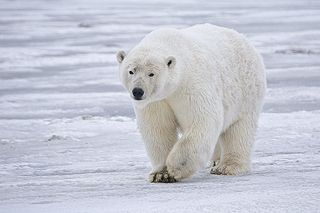
\includegraphics[width=0.5\textwidth]{polar_bear.jpg}
		\end{center}
		\caption{Polar Bear.}
		\label{figcaption}
	\end{figure}
	
	{\itshape Hint: (\texttt{figure} is a floating environment that gets put where it nicely fits the page layout. 
		The optional argument says which positions are acceptable for the float: 
		\underline{t}op/\underline{b}ottom of a page, \underline{h}ere, and on a separate \underline{p}age of floats.)}
	
	\begin{figure}[tbhp]
		\begin{center}
			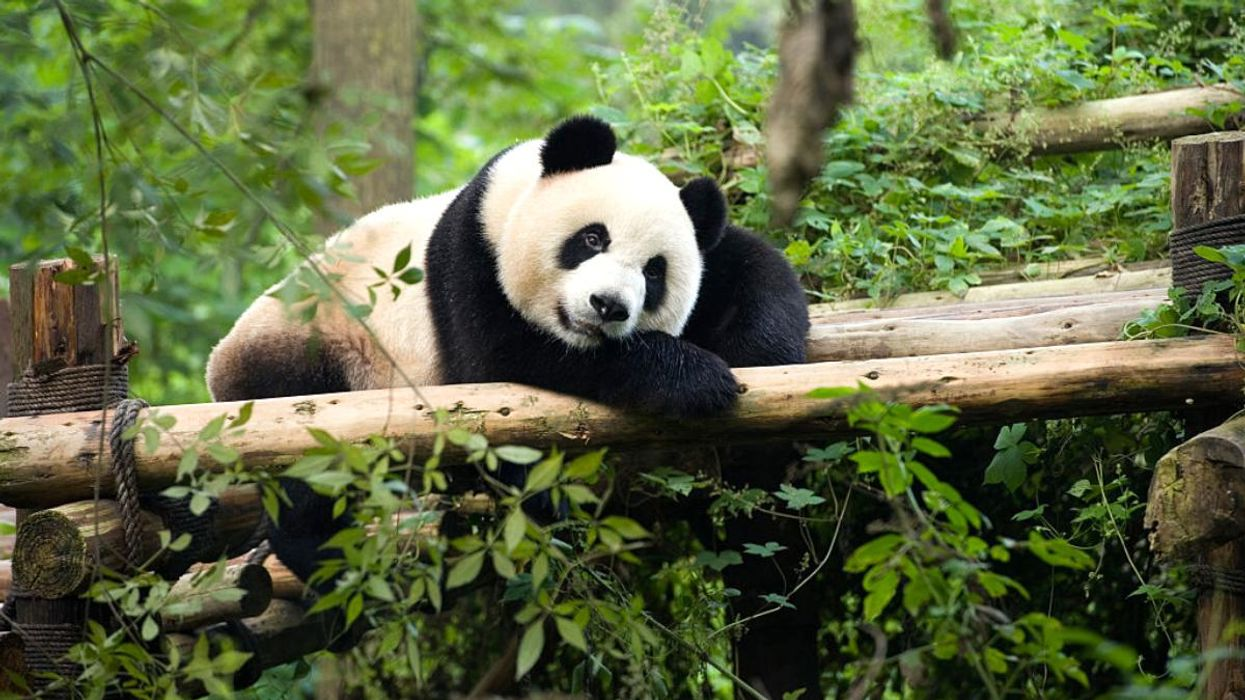
\includegraphics[width=0.5\textwidth]{giant_panda.jpg}
		\end{center}
		\caption{Giant Panda.}
	\end{figure}
\end{document}